% !TeX spellcheck = en_US
\addscenariosection{1}{Clash Scenario}{Bloody Grail}{\images/bloody-grail.png}

\begin{multicols*}{2}

\textbf{Author:} Re4XN

\textbf{Source:} \href{https://discord.com/channels/740870068178649108/1239631918643941509}{Archon Studios Discord}

\textit{A lady clad in dark robes visits you in your dreams, offering you a golden chalice filled with blood-red wine. Waking up in a cold sweat, you decide to embark on a quest to find this unholy artifact.}

\subsection*{\MakeUppercase{Scenario Length}}
This Scenario is played over 13 Rounds.

\subsection*{\MakeUppercase{Player Setup}}
\textbf{Player Count:} 2 or 4

\textbf{Starting Resources:} 13 \svg{gold}, 2 \svg{building_materials}, 1 \svg{valuables}

\textbf{Starting Income:} 10 \svg{gold}, 0 \svg{building_materials}, 0 \svg{valuables}

\textbf{Starting Units:}
\begin{itemize}
  \item A Few \bronze\ Units with the \textit{highest} Recruitment cost
  \item A Pack of \bronze\ Units with the \textit{lowest} Recruitment cost
\end{itemize}

\textbf{Town Buildings:} \bronze\ Dwelling

\textbf{Map Tile Pool:} Each player takes 2 random Far (II--III) Map Tiles, one of which must contain a Settlement

\subsection*{\MakeUppercase{Map Setup}}
Take the following Map Tiles and arrange them as shown in the Scenario map layout:

\textbf{For a 2-player Scenario:}
\begin{itemize}
  \item 2 × Starting (I) Map Tile
  \item 4 × Near (IV--V) Map Tile, all of which must contain an Obelisk
  \item 4 × Far (II--III) Map Tile, 2 of which must contain a Settlement
  \item 1 × Center (VI--VII) Map Tile, which must contain the Grail Field
\end{itemize}

\textbf{For a 4-player Scenario:}
\begin{itemize}
  \item 4 × Starting (I) Map Tile
  \item 6 × Near (IV--V) Map Tile, 4 of which must contain an Obelisk
  \item 8 × Far (II--III) Map Tile, 4 of which must contain a Settlement
  \item 1 × Center (VI--VII) Map Tile, which must contain the Grail Field
\end{itemize}

\textbf{\MakeUppercase{Note:}} Before placing the Near Tiles, separate them into 2 piles (with and without an Obelisk). Place them alternately so that the Tiles with an Obelisk are not placed adjacent to each other.

\subsection*{\MakeUppercase{Victory Conditions}}
To win the Scenario, a Hero must obtain the Grail Token and bring it to their Faction Town.

\subsection*{\MakeUppercase{Defeat Conditions}}
If the Grail is not obtained at least once by the end of the \nth{13} Round, the game ends, and all players lose the Scenario.

If the Grail Token has been obtained, the players gain additional time (until the end of the \nth{16} Round) to bring the Grail to their Faction's Town. Otherwise, all players lose the Scenario.

\columnbreak
\subsection*{\MakeUppercase{Timed Events}}

\textbf{\nth{6}, \nth{9} and \nth{12} Rounds:}
\begin{itemize}
  \item Remove all Black Cubes from every Water Wheel and Windmill on the map.
  \item All players possessing the title of ``\textcolor{cobalt}{Grail Knight}'' gain \svg{morale_positive}.
  \item All players who do not possess a title gain 2 \svg{morale_negative}.
\end{itemize}

\subsection*{\MakeUppercase{Additional Rules}}
Before this Scenario:

\begin{itemize}
  \item Split the Artifact Deck by rarity into 3 separate Decks (Minor, Major, and Relic). A player may gain only Minor Artifacts on Starting or Far Tiles, Minor or Major Artifacts on Near Tiles, and Major or Relic Artifacts on Center Tiles.
\end{itemize}

During this Scenario:

\begin{itemize}
  \item When a player Visits an Obelisk, they \textit{must} resolve one of the following effects:
  \begin{enumerate}[leftmargin=15pt]
    \item \textbf{[Cleanse]} The player receives one of the following boons, depending on how many Obelisks they have Visited:
    \begin{enumerate}
      \item \textbf{[1st Obelisk]} You gain a Secondary Hero. Place their model on this Field. If you already have one, gain 6 \svg{gold} instead. Then, choose one enemy player to discard 1 random Card from their hand.
      \item \textbf{[2nd Obelisk]} Increase your \svg{gold}, \svg{building_materials}, or \svg{valuables} income by 1 step.
      \item \textbf{[3rd Obelisk]} Roll 2 \svg{treasure} and choose 1 to resolve; then, gain \svg{morale_positive} and \svgeven{movement}.
      \item \textbf{[4th Obelisk]} Remove up to 4 Cards from your hand, except Statistic Cards; then, search each corresponding Deck for a Card of your choice and put it in your hand.
    \end{enumerate}
    \item \textbf{[Sacrifice]} Remove a * Faction Unit Card from your Unit Deck in exchange for:
    \begin{enumerate}
      \item *\bronze\: Gain 6 \svg{gold}, 3 \svg{building_materials}, and 1 \svg{valuables}. Additionally, if the Unit Card was on the Pack side, \textbf{Search (4)} the Minor Artifact Deck.
      \item *\silver\: Gain 12 \svg{gold}, 6 \svg{building_materials}, and 2 \svg{valuables}. Additionally, if the Unit Card was on the Pack side, \textbf{Search (3)} the Major Artifact Deck.
      \item *\golden\: Gain 18 \svg{gold}, 9 \svg{building_materials}, and 3 \svg{valuables}. Additionally, \textbf{Search (2)} the Relic Card Deck. Finally, if the Unit Card was on the Pack side, \textbf{Search (2)} the \azure\ Unit Deck; you may Recruit one of these Units for half the cost (rounded down).
    \end{enumerate}
  \end{enumerate}
  \item A player that chooses \textbf{Sacrifice} at an Obelisk gains the title of ``\textcolor{darkcandyapplered}{Blood Knight}.'' Place a red Faction Cube on their Hero portrait to mark this effect. A \textcolor{darkcandyapplered}{Blood Knight} may never choose the \textbf{Cleanse} option when Visiting an Obelisk.
  \item A player that chooses \textbf{Cleanse} at an Obelisk gains the title of ``\textcolor{cobalt}{Grail Knight}.'' Place a blue Faction Cube on their Hero portrait to mark this effect. A \textcolor{cobalt}{Grail Knight} may never choose the \textbf{Sacrifice} option when Visiting an Obelisk.
  \item When a player chooses \textbf{Sacrifice} at an Obelisk, place a number of Faction Cubes on the sacrificed Unit Card and on the Obelisk Field equivalent to the number of times the player has chosen the \textbf{Sacrifice} option. For example, if the player is sacrificing for the second time, place 2 Faction Cubes on the Unit Card and 2 Faction Cubes on the Obelisk Field.
  \item A player who possesses the title of ``\textcolor{cobalt}{Grail Knight}'' may, after Visiting an Obelisk, Recruit an enemy Unit sacrificed at that Obelisk for half the cost (rounded down); if a Pack was sacrificed, the player may choose to Recruit Few instead.
  \item If a Unit Recruited at an Obelisk is defeated, remove it.
  \item A player who possesses no title or the title of ``\textcolor{darkcandyapplered}{Blood Knight}'' may not use the Diplomacy Ability Card. If a player who possesses no title or the title of ``\textcolor{darkcandyapplered}{Blood Knight}'' draws the Diplomacy Ability Card, they may show it to the other players, then discard it and draw a new Ability Card in its stead.
  \item A player who possesses the title of ``\textcolor{cobalt}{Grail Knight}'' may not use the Diplomacy Ability Card to Recruit Neutral \azure\ Units.
  \item Whenever an Astrologers Proclaim or Event Card that allows you to Recruit Neutral Units is drawn, ignore it and draw a new Astrologers Proclaim or Event Card.
  \item Players can use their Deck of Might \& Magic when paying gold to defend their Faction Town.
  \item Ignore Combat encounters on the Field with the Grail.
  \item Players may not Visit the Field with the Grail Token unless they have already Visited at least two Obelisks or the Grail Token has been taken by any Hero at least once.
  \item To obtain the Grail Token, a player’s Hero must spend 2 \svgeven{movement} on the Field with the Grail.
  \item If a player does not possess the title of ``\textcolor{darkcandyapplered}{Blood Knight},'' they must Remove a Faction Unit Card from their Unit Deck immediately after obtaining the Grail Token. This effect can only occur once per player.
  \item If another Hero defeats the Hero with the Grail Token, they also take the Grail Token.
  \item If a Hero with the Grail Token Surrenders, the Grail Token is placed on the hex where the Hero Surrendered.
  \item If a Neutral army defeats the Hero with the Grail Token, the Grail Token is placed on the Field where the Hero was defeated.
  \item If a Hero with the Grail Token casts Town Portal or uses the Inferno Faction Castle Gate building, the Grail Token is placed on the hex where the Spell was cast or the building used.
  \item The Grail Token behaves like a Permanent Card that does not count towards your hand limit and cannot be discarded; it grants the following effect when played: ``$\infty$ Once during each Combat, if the Hero is a \textcolor{darkcandyapplered}{Blood Knight}, discard a Card to remove up to 2 \svg{damage-red} from your Units and assign it to enemy Units.''
  \item A Hero with the Grail Token who possesses the title of ``\textcolor{cobalt}{Grail Knight}'' may pay 10 \svg{gold} or 3 \svg{valuables} at any Temple map location to cleanse the Grail. Place a blue Faction Cube on the Grail Token to mark this effect.
  \item Once cleansed, the Grail Token behaves like a Permanent Card that does not count towards your hand limit and cannot be discarded; it grants the following effect when played: ``$\infty$ Once during each Combat Round, if the Hero is a \textcolor{cobalt}{Grail Knight}, discard a Card to remove up to 2 \svg{damage-red} from your Units.''
\end{itemize}

\vspace*{\fill}

\begin{center}
  \transparent{0.2}{
\includegraphics[width=0.5\linewidth, keepaspectratio]{\art/bless.png}}
\end{center}

\vspace*{\fill}

\end{multicols*}

\begin{tikzpicture}[overlay]
  \node(bg)[anchor=center, opacity=0.07, xshift=0em, yshift=-25em] at (current page.south) {
    
\includegraphics[width=1.2\paperwidth, keepaspectratio]{\art/quiet_eye_of_the_dragon.png}
  };
  \centering
  \node at (4.5, -5) {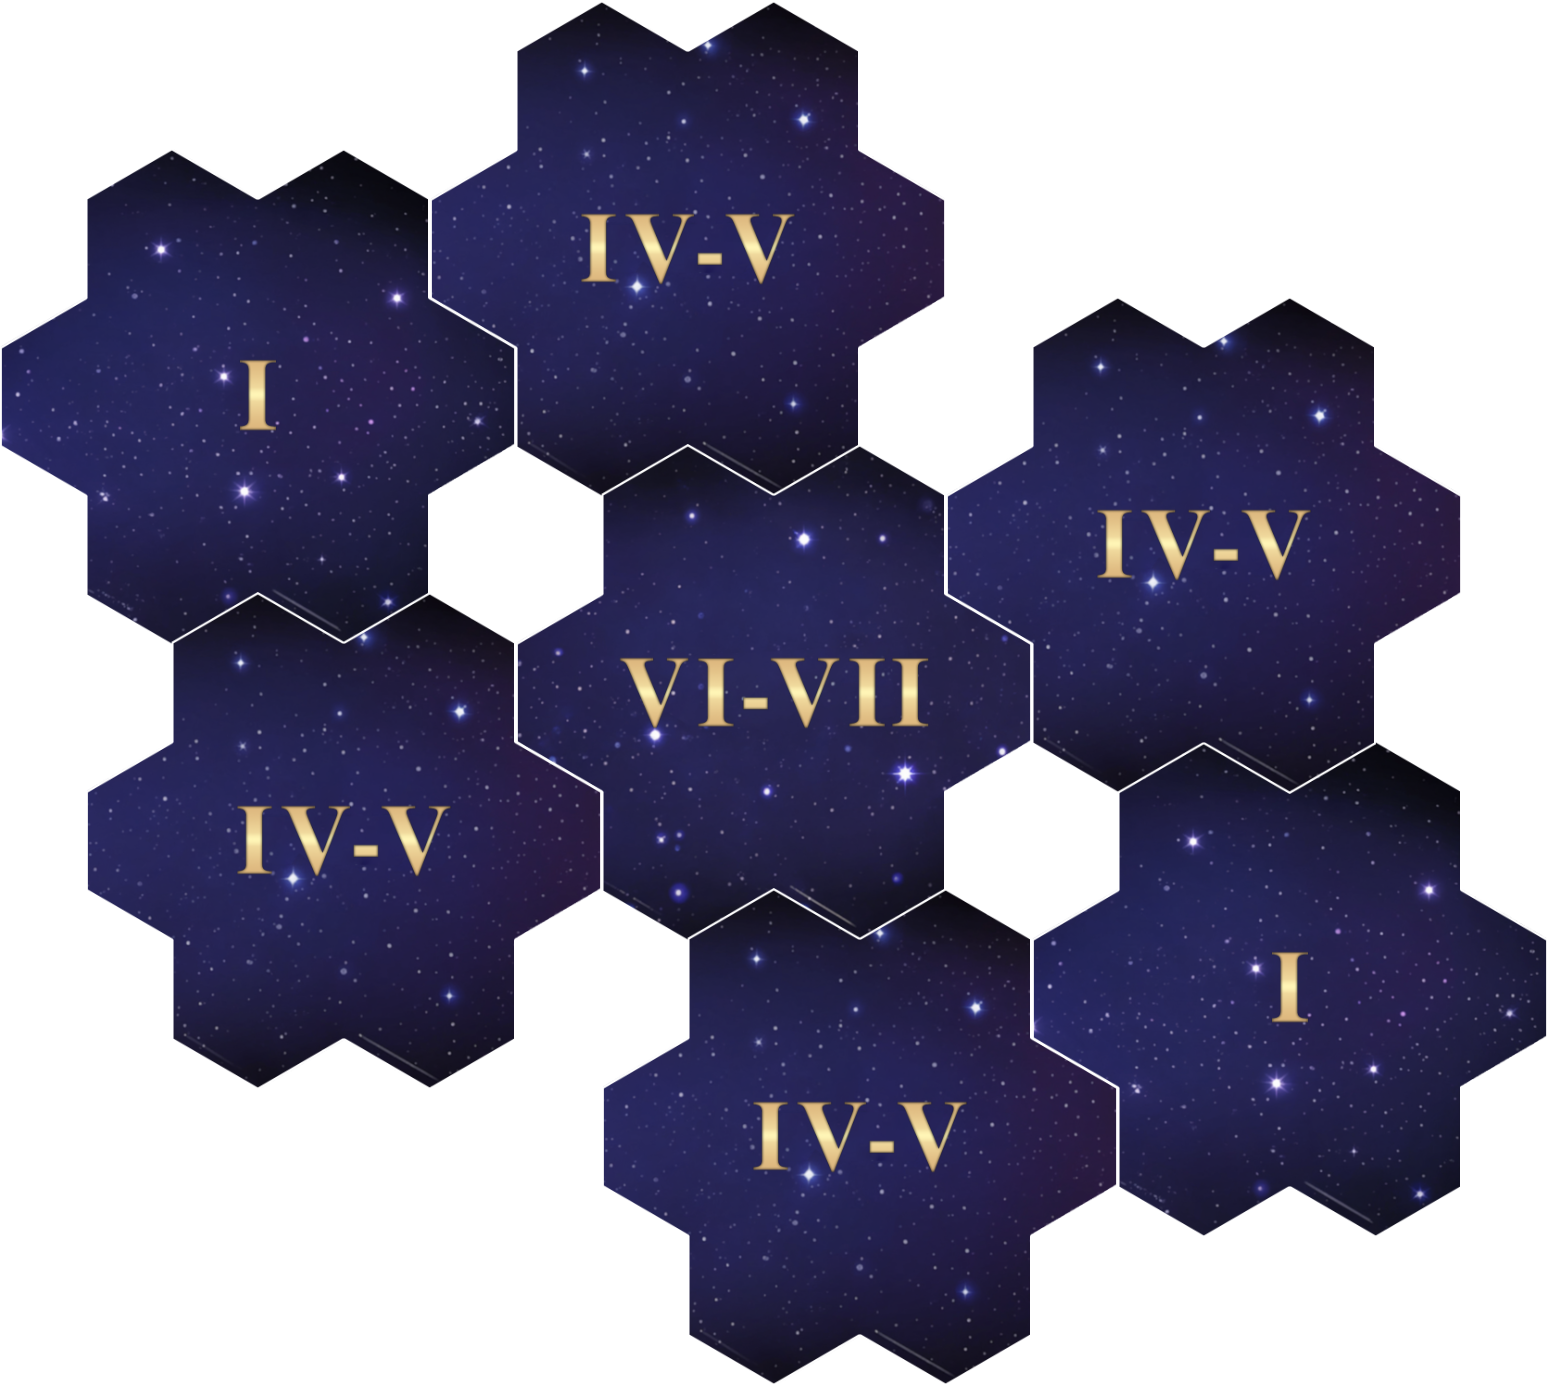
\includegraphics[scale=0.165]{\maps/bloody-grail-2p.png}};
  \node at (4.5, -10) {\footnotesize{\textbf{\MakeUppercase{2-PLAYER SCENARIO}}}};
  \node at (12.1, -14) {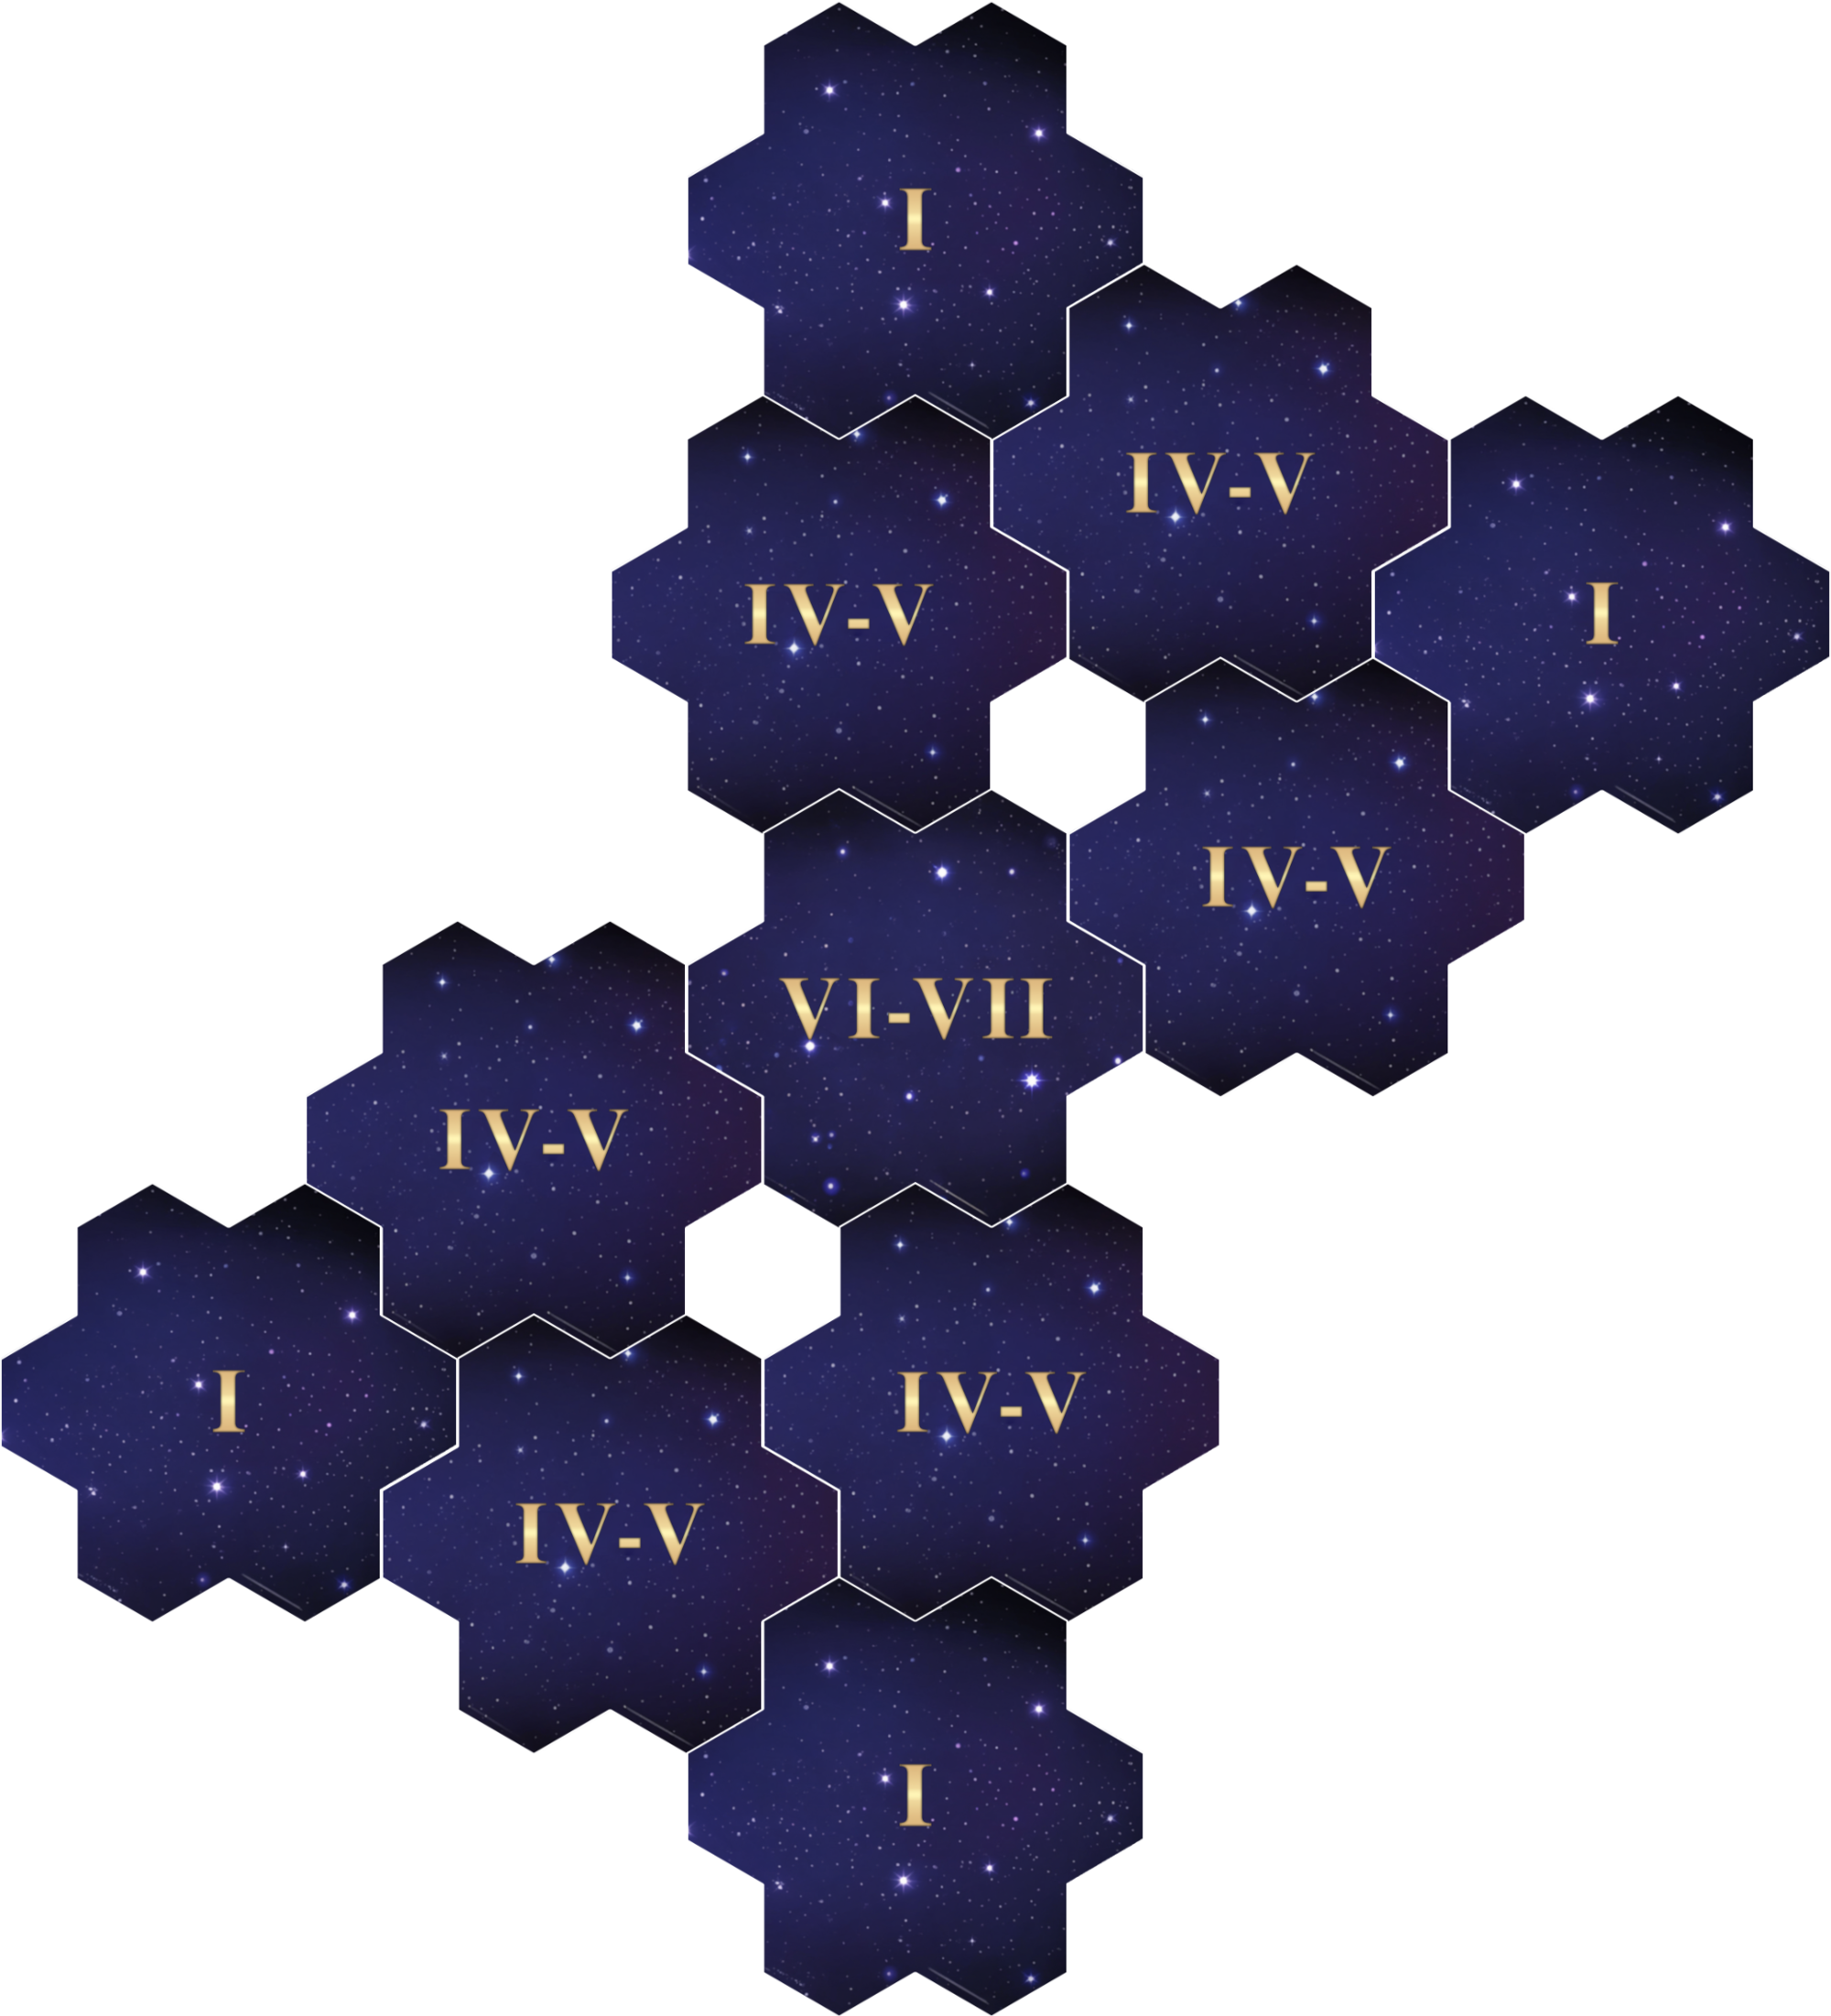
\includegraphics[scale=0.165]{\maps/bloody-grail-4p.png}};
  \node at (12.1, -21.6) {\footnotesize{\textbf{\MakeUppercase{4-PLAYER SCENARIO}}}};
\end{tikzpicture}
